\documentclass{standalone}
\usepackage{graphicx}	
\usepackage{amssymb, amsmath}
\usepackage{color}

\usepackage{tikz}
\usetikzlibrary{intersections, backgrounds}
\usepackage{pgfmath}

\definecolor{light}{RGB}{220, 188, 188}
\definecolor{mid}{RGB}{185, 124, 124}
\definecolor{dark}{RGB}{143, 39, 39}
\definecolor{highlight}{RGB}{180, 31, 180}
\definecolor{gray10}{gray}{0.1}
\definecolor{gray20}{gray}{0.2}
\definecolor{gray30}{gray}{0.3}
\definecolor{gray40}{gray}{0.4}
\definecolor{gray60}{gray}{0.6}
\definecolor{gray70}{gray}{0.7}
\definecolor{gray80}{gray}{0.8}
\definecolor{gray90}{gray}{0.9}
\definecolor{gray95}{gray}{0.95}

\newcommand*{\offset}{0.025}

\begin{document}

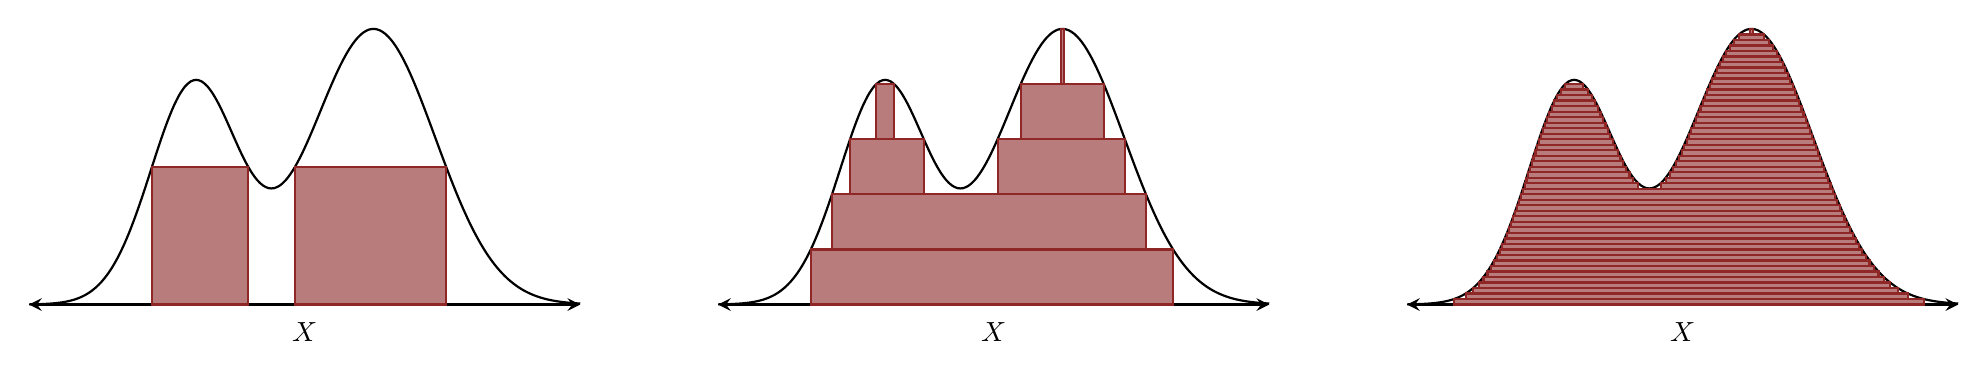
\begin{tikzpicture}[scale=0.35, thick, 
declare function={ g(\x) = 10 * exp(-0.1 * (\x - 2.5) * (\x - 2.5)) 
                          + 8 * exp(-0.2 * (\x + 4) * (\x + 4));},
]

  \draw [<->, >=stealth, line width=1] (-35, 0) -- +(20, 0);
  \node[] at (-25, -1) { $X$ };

  \draw[domain=-10:10, smooth, samples=100, variable=\x] 
    plot ({\x - 25},{g(\x)});

  \def\lower{{-5.53807575979178, -0.347476353587045}}
  \def\upper{{-2.04943175151915, 5.13276260434322}}
  \def\height{{5, 5}}
  \foreach \n in {0, 1} {
    \pgfmathparse{\lower[\n]}\edef\l{\pgfmathresult}
    \pgfmathparse{\upper[\n]}\edef\u{\pgfmathresult}
    \pgfmathparse{\height[\n]}\edef\h{\pgfmathresult}
    \filldraw[fill=mid, draw=dark] (\l - 25, 0) rectangle (\u - 25, \h);
  }

  %
  \draw [<->, >=stealth, line width=1] (-10, 0) -- +(20, 0);
  \node[] at (0, -1) { $X$ };
  
  \draw[domain=-10:10, smooth, samples=100, variable=\x] 
    plot ({\x},{g(\x)});
    
  \def\lower{{2.45620023288914, 0.982966700595389, -4.25598715686893, 0.144781471736031, -5.20844836681707, -5.86471401624836, -6.63391991706263}}
  \def\upper{{2.53931923870967, 3.99378547575161, -3.61061303287104, 4.76012889108101, -2.53476722607382, 5.52702983384044, 6.51177837536601}}
  \def\height{{10, 8, 8, 6, 6, 4, 2}}
  \foreach \n in {0, 1, ..., 6} {
    \pgfmathparse{\lower[\n]}\edef\l{\pgfmathresult}
    \pgfmathparse{\upper[\n]}\edef\u{\pgfmathresult}
    \pgfmathparse{\height[\n]}\edef\h{\pgfmathresult}
    \filldraw[fill=mid, draw=dark] (\l, 0) rectangle (\u, \h);
  }

  %
  \draw [<->, >=stealth, line width=1] (15, 0) -- +(20, 0);
  \node[] at (25, -1) { $X$ };
  
  \draw[domain=-10:10, smooth, samples=100, variable=\x] 
    plot ({\x + 25},{g(\x)});
    
  \def\lower{{2.45620023288914, 2.04449892268754, 1.85423500760145, 1.70535396976636, 1.57745533255511, 1.46251260020328, 1.35647530370423, 1.25689591750225, 1.1621853386526, 1.07114291618873, 0.982966700595389, -4.25598715686893, 0.896940981968987, -4.42419211531729, 0.812598082966065, -4.54984963576119, 0.729364024661376, -4.65598568604677, 0.646862098890963, -4.75039709758729, 0.564692455014686, -4.83698477317131, 0.482456574190068, -4.91796479131718, 0.399808318352599, -4.99473802077879, 0.316285641779779, -5.06825225760651, 0.231433641226938, -5.13932901437213, 0.144781471736032, -5.20844836681707, 0.0556181869682566, -5.27606920953583, -0.0368650158648903, -5.34255321956028, -0.133693584959152, -5.40823344287711, -0.236459329679247, -5.47331802327085, -0.347476353587045, -5.53807575979178, -0.470686051404074, -5.6027366520747, -0.613744473839886, -5.66754716664442, -0.797169331069228, -5.73266956142296, -5.79832249764835, -5.86471401624836, -5.93207463746366, -6.00063966391276, -6.0707302759251, -6.14251566475609, -6.2164194845952, -6.29280531315853, -6.37212952981502, -6.45494224964215, -6.54192086811663, -6.63391991706263, -6.73198834420715, -6.83765760135063, -6.95289004297407, -7.08058153073824, -7.22507993515209, -7.39360612438913, -7.59922170543148, -7.87054662812817, -8.29494674387808}}
  \def\upper{{2.53931923870967, 2.95004288525657, 3.13915746727364, 3.28673863712856, 3.41319157493227, 3.5265039273953, 3.63068141944489, 3.72811990809431, 3.82044700277268, 3.90873454943037, 3.99378547575161, -3.61061303287104, 4.07627319527994, -3.43464262589641, 4.15662231525223, -3.300522891001, 4.23525219627284, -3.18520692892386, 4.31249023094514, -3.08074938607857, 4.38861296851085, -2.98308928396937, 4.46385974534017, -2.88993388777489, 4.53844278557131, -2.79967189985471, 4.61255471812897, -2.71104227837155, 4.68638598674635, -2.62305248222278, 4.76012889108101, -2.53476722607382, 4.83395077597826, -2.44523609949886, 4.90794242465174, -2.35345424486579, 4.98230995288815, -2.25812925936038, 5.05719878141711, -2.15762099856955, 5.13276260434322, -2.04943175151915, 5.20917157578815, -1.92960165400345, 5.28659642018204, -1.79033550406882, 5.36528155154261, -1.6110541903249, 5.44533645203389, 5.52702983384044, 5.61060208391482, 5.69632972641349, 5.78452754660386, 5.87555856962056, 5.96984725009405, 6.06783633606913, 6.17025025116965, 6.27771954095572, 6.39117822959331, 6.51177837536601, 6.64101006408536, 6.78086241613403, 6.93408083698173, 7.10461945340072, 7.29855605606336, 7.52566329803178, 7.80416444060818, 8.17351384684708, 8.75459055459849}}
  \def\height{{10, 9.8, 9.6, 9.4, 9.2, 9, 8.8, 8.6, 8.4, 8.2, 8, 8, 7.8, 7.8, 7.6, 7.6, 7.4, 7.4, 7.2, 7.2, 7, 7, 6.8, 6.8, 6.6, 6.6, 6.4, 6.4, 6.2, 6.2, 6, 6, 5.8, 5.8, 5.6, 5.6, 5.4, 5.4, 5.2, 5.2, 5, 5, 4.8, 4.8, 4.6, 4.6, 4.4, 4.4, 4.2, 4, 3.8, 3.6, 3.4, 3.2, 3, 2.8, 2.6, 2.4, 2.2, 2, 1.8, 1.6, 1.4, 1.2, 1, 0.8, 0.6, 0.4, 0.2}}
  \foreach \n in {0, 1, ..., 68} {
    \pgfmathparse{\lower[\n]}\edef\l{\pgfmathresult}
    \pgfmathparse{\upper[\n]}\edef\u{\pgfmathresult}
    \pgfmathparse{\height[\n]}\edef\h{\pgfmathresult}
    \filldraw[fill=mid, draw=dark] (\l + 25, 0) rectangle (\u + 25, \h);
  }
   
\end{tikzpicture}

\end{document}  